\documentclass[xcolor=x11names, aspectratio=169,usenames,dvipsnames]{beamer}
\usepackage[british]{babel}
\usepackage{amsmath}
\usepackage{amssymb}
\usepackage{amsfonts}
\usepackage{mathpazo}
\usepackage{enumerate}
\usepackage{array,booktabs}
\usepackage{tikz}
\usepackage{mathdots}
\usepackage{verbatim}
\usepackage{multirow}
\usepackage{tabularx}
\usetikzlibrary{overlay-beamer-styles,shadows,matrix,backgrounds,patterns,arrows,decorations.markings,shapes,positioning,calc,chains,scopes,fit}
\usepackage{caption}

\usetheme[titleformat title=regular,titleformat frame=regular,titleformat section=allcaps,numbering=fraction]{metropolis}

\author[Felix Kußmaul]{\large Felix Kußmaul\inst{1}}
\title[FMSync]{\Large FMSync}
\subtitle{\normalsize An Open Source Solution for Synchronising Distributed Archaeological Databases in a Centralised Open Access System}
\institute[Cologne]{\inst{1} Archäologisches Institut, Universität zu Köln}
\date[\today]{\vspace*{1em}CAA 2018, Tübingen\\[.5em] 21 March 2018\vspace*{1em}}

\titlegraphic{
    \tikz[overlay,remember picture]
        \node[xshift=-17em,yshift=13em,at=(current page.south east), anchor=north west] {
            
\includegraphics[width=0.55\textwidth]{img/uni.eps}
        };
}
\usepackage{pdfrender}

\newcommand{\red}[1]{\textcolor{red}{#1}}
\newcommand{\orange}[1]{\textcolor{orange}{#1}}
\newcommand{\green}[1]{\textcolor{markgreen}{#1}}
\newcommand{\textgreen}[1]{\textcolor{textgreen}{#1}}
\newcommand{\blue}[1]{\textcolor{textblue}{#1}}
\newcommand{\gray}[1]{\textcolor{gray}{#1}}

\newcolumntype{R}{>{\centering\raggedleft\arraybackslash}X}
\newcolumntype{L}{>{\centering\raggedright\arraybackslash}X}
\newcolumntype{C}{>{\centering\arraybackslash}X}

\usepackage[style=authortitle-comp,backend=biber]{biblatex}
\addbibresource{caa.bib}
\renewcommand*{\bibfont}{\small}

\setbeamercovered{transparent}

\newcommand{\textsb}[1]{{\fontfamily{cmss}\fontseries{sbc}\fontshape{n}\selectfont #1}}

\setbeamertemplate{enumerate items}[square]

\setbeamertemplate{footline}
{
\hbox{%
  \begin{beamercolorbox}[wd=.26\paperwidth,ht=2.7ex,dp=1.2ex,center]{author in head/foot}%
    \usebeamerfont{author in head/foot}\insertshortauthor\ (\insertshortinstitute)
  \end{beamercolorbox}%
  \begin{beamercolorbox}[wd=.40\paperwidth,ht=2.7ex,dp=1.2ex,center]{author in head/foot}%
    \usebeamerfont{title in head/foot}\insertshorttitle:\ \textbf{\insertsection}
  \end{beamercolorbox}%
  \begin{beamercolorbox}[wd=.36\paperwidth,ht=2.7ex,dp=1.2ex,center]{author in head/foot}%
    \usebeamerfont{date in head/foot}\insertshortdate\hfill\insertframenumber/\inserttotalframenumber\strut
  \end{beamercolorbox}}
  \vskip0pt%
}

\tikzset{
  invisible/.style={opacity=0},
  visible on/.style={alt={#1{}{invisible}}},
  alt/.code args={<#1>#2#3}{%
    \alt<#1>{\pgfkeysalso{#2}}{\pgfkeysalso{#3}} % \pgfkeysalso doesn't change the path
  },
}

\newcommand{\printSectionYes}{\AtBeginSection[]
{
 \begin{frame}{Agenda}
 \tableofcontents[sectionstyle=show/shaded,
 					subsectionstyle=show/shaded/hide]
 \end{frame}
}}

\tikzset{onslide/.code args={<#1>#2}{%
  \only<#1>{\pgfkeysalso{#2}}%
}}

\setbeamertemplate{section in toc shaded}[default][50]

\setbeamertemplate{subsection in toc shaded}[default][50]

\makeatletter
\patchcmd{\beamer@sectionintoc}{\vskip1.5em}{\vskip0.5em}{}{}
\makeatother

\makeatletter
\newcommand\footnoteref[1]{\protected@xdef\@thefnmark{\ref{#1}}\@footnotemark}
\makeatother

\setbeamertemplate{bibliography item}{%
  \ifboolexpr{ test {\ifentrytype{book}} or test {\ifentrytype{mvbook}}
    or test {\ifentrytype{collection}} or test {\ifentrytype{mvcollection}}
    or test {\ifentrytype{reference}} or test {\ifentrytype{mvreference}} }
    {\setbeamertemplate{bibliography item}[book]}
    {\ifentrytype{online}
       {\setbeamertemplate{bibliography item}[online]}
       {\setbeamertemplate{bibliography item}[article]}}%
  \usebeamertemplate{bibliography item}}
  
\defbibenvironment{bibliography}
  {\list{}
     {\settowidth{\labelwidth}{\usebeamertemplate{bibliography item}}%
      \setlength{\leftmargin}{\labelwidth}%
      \setlength{\labelsep}{\biblabelsep}%
      \addtolength{\leftmargin}{\labelsep}%
      \setlength{\itemsep}{\bibitemsep}%
      \setlength{\parsep}{\bibparsep}}}
  {\endlist}
  {\item}
  
%%% DEFINE DOCUMENT SHAPE
% taken from manual
\makeatletter
\pgfdeclareshape{document}{
\inheritsavedanchors[from=rectangle] % this is nearly a rectangle
\inheritanchorborder[from=rectangle]
\inheritanchor[from=rectangle]{center}
\inheritanchor[from=rectangle]{north}
\inheritanchor[from=rectangle]{south}
\inheritanchor[from=rectangle]{west}
\inheritanchor[from=rectangle]{east}
% ... and possibly more
\backgroundpath{% this is new
% store lower right in xa/ya and upper right in xb/yb
\southwest \pgf@xa=\pgf@x \pgf@ya=\pgf@y
\northeast \pgf@xb=\pgf@x \pgf@yb=\pgf@y
% compute corner of ‘‘flipped page’’
\pgf@xc=\pgf@xb \advance\pgf@xc by-5pt % this should be a parameter
\pgf@yc=\pgf@yb \advance\pgf@yc by-5pt
% construct main path
\pgfpathmoveto{\pgfpoint{\pgf@xa}{\pgf@ya}}
\pgfpathlineto{\pgfpoint{\pgf@xa}{\pgf@yb}}
\pgfpathlineto{\pgfpoint{\pgf@xc}{\pgf@yb}}
\pgfpathlineto{\pgfpoint{\pgf@xb}{\pgf@yc}}
\pgfpathlineto{\pgfpoint{\pgf@xb}{\pgf@ya}}
\pgfpathclose
% add little corner
\pgfpathmoveto{\pgfpoint{\pgf@xc}{\pgf@yb}}
\pgfpathlineto{\pgfpoint{\pgf@xc}{\pgf@yc}}
\pgfpathlineto{\pgfpoint{\pgf@xb}{\pgf@yc}}
\pgfpathlineto{\pgfpoint{\pgf@xc}{\pgf@yc}}
}
}
\makeatother


%\setbeamertemplate{title page}{%
%\begin{tikzpicture}[remember picture,overlay]
%\fill[orange]
%  ([yshift=15pt]current page.west) rectangle (current page.south east);
%\node[anchor=east] 
%  at ([yshift=-50pt]current page.north east) (author)
%  {\parbox[t]{.6\paperwidth}{\raggedleft%
%    \usebeamerfont{author}\textcolor{orange}{%
%    \textpdfrender{
%    TextRenderingMode=FillStroke,
%    FillColor=orange,
%    LineWidth=.1ex,
%    }{\insertauthor}}}};
%\node[anchor=north east] 
%  at ([yshift=-70pt]current page.north east) (institute)
%  {\parbox[t]{.78\paperwidth}{\raggedleft%
%    \usebeamerfont{institute}\textcolor{gray}{\insertinstitute}}};
%\node[anchor=south west] 
%  at ([yshift=20pt]current page.west) (logo)
%  {\parbox[t]{.19\paperwidth}{\raggedleft%
%    \usebeamercolor[fg]{titlegraphic}\inserttitlegraphic}};
%\node[anchor=east]
%  at ([yshift=-10pt,xshift=-20pt]current page.east) (title)
%  {\parbox[t]{\textwidth}{\raggedleft%
% \usebeamerfont{author}\textcolor{white}{%
%    \textpdfrender{
%    TextRenderingMode=FillStroke,
%    FillColor=white,
%    LineWidth=.1ex,
%    }{\inserttitle}}}};
%\node[anchor=east]
%  at ([yshift=-60pt,xshift=-20pt]current page.east) (subtitle)
%  {\parbox[t]{.6\paperwidth}{\raggedleft\usebeamerfont{subtitle}\textcolor{black}{\insertsubtitle}}};
%\end{tikzpicture}
%}
\definecolor{morange}{HTML}{FF8200}
\metroset{block=fill}

\setbeamercolor{background canvas}{bg=white}
 
\begin{document}

\begin{frame}[plain]
\titlepage
\end{frame}

\section{Motivation}

\begin{frame}{Before FMSync: Sharing Data}
\begin{figure}
	\begin{tikzpicture}
\only<1-4>{\draw[thick, dashed,gray] (5.75,-3) -- (5.75,3);}
\only<5->{\draw[thick, dashed,gray] (5.75,-4.7) -- (5.75,2);}
\node (pc) at (0,0) {\reflectbox{
\includegraphics[width=2cm]{img/pc.jpg}}};
\node[right of=pc, node distance=3em] (db) {
\includegraphics[width=2em]{img/db}};
\only<2->{
	\node[right of=pc, node distance=4cm](usb) {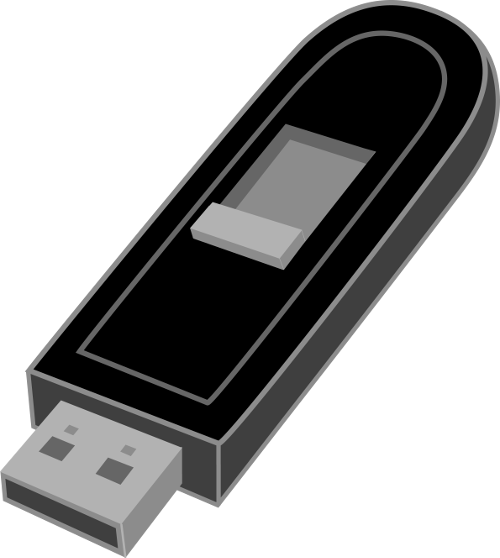
\includegraphics[width=3em]{img/usb}};
	\node[below right of=usb, node distance=1em] (db2) {
\includegraphics[width=1em]{img/db}};
	\draw[arrows=-latex,ultra thick] (db) -- node [above] {\small{copy}} (usb);
}
\only<3->{
	\node[right of=usb, node distance=3.5cm](usb2) {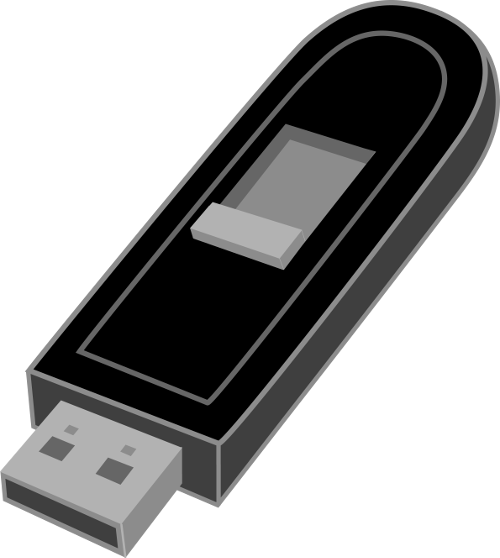
\includegraphics[width=3em]{img/usb}};
	\node[below right of=usb2, node distance=1em] (db4) {
\includegraphics[width=1em]{img/db}};
	\draw[arrows=-latex,ultra thick] (usb) -- node[above] (box) {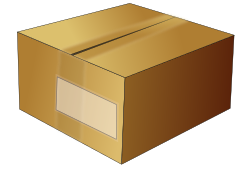
\includegraphics[width=4em]{img/box}} (usb2);
}
\node[right of=pc, node distance=11.5cm] (pc2) {
\includegraphics[width=2cm]{img/pc.jpg}};
\node[left of=pc2, node distance=3em] (db3) {
\includegraphics[width=2em]{img/db2}};
\only<4->{
	\node[below left of=db3, node distance=1em] (dbb3) {
\includegraphics[width=2em]{img/db}};
	\draw[arrows=-latex,ultra thick] (usb2) -- node [above] {\small{copy}} (dbb3);
}
\only<5->{
	\node (pcb) at (0,-3.3) {\reflectbox{
\includegraphics[width=2cm]{img/pc.jpg}}};
	\node[right of=pcb, node distance=3em] (dbb) {
\includegraphics[width=2em]{img/db}};
	\node[below right of=dbb, node distance=1em] (dbb3b) {
\includegraphics[width=2em]{img/db2}};
	\node[right of=pcb, node distance=4cm](usbb) {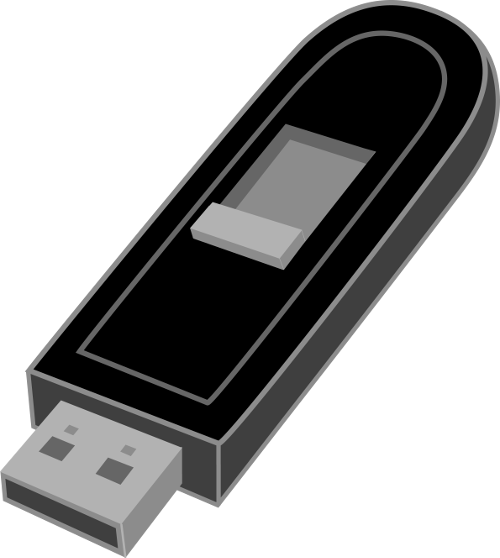
\includegraphics[width=3em]{img/usb}};
	\node[below right of=usbb, node distance=1em] (db2b) {
\includegraphics[width=1em]{img/db2}};
	\draw[arrows=-latex,ultra thick] (usbb) -- node [above] {\small{copy}} (dbb3b);
	\node[right of=usbb, node distance=3.5cm](usb2b) {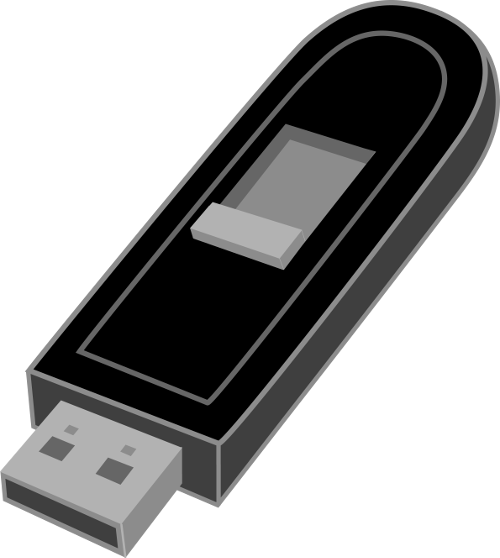
\includegraphics[width=3em]{img/usb}};
	\node[below right of=usb2b, node distance=1em] (db4b) {
\includegraphics[width=1em]{img/db2}};
	\draw[arrows=-latex,ultra thick] (usb2b) -- node[above] (boxb) {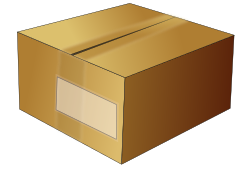
\includegraphics[width=4em]{img/box}} (usbb);
	\node[right of=pcb, node distance=11.5cm] (pc2b) {
\includegraphics[width=2cm]{img/pc.jpg}};
	\node[left of=pc2b, node distance=3em] (db3b) {
\includegraphics[width=2em]{img/db2}};
	\node[below left of=db3b, node distance=1em] {
\includegraphics[width=2em]{img/db}};
	\draw[arrows=-latex,ultra thick] (db3b) -- node [above] {\small{copy}} (usb2b);
}
\end{tikzpicture}
\end{figure}
\end{frame}

\begin{frame}{Before FMSync: Publishing Data}
\begin{figure}
	\vspace{-2.5em}
	\begin{tikzpicture}
	\draw[thick, dashed,gray] (5.75,-3) -- (5.75,3);
	\node (pc) at (0,0) {\reflectbox{
\includegraphics[width=2cm]{img/pc.jpg}}};
	\node[right of=pc, node distance=3em] (db) {
\includegraphics[width=2em]{img/db}};
	\node[right of=pc, node distance=11.5cm] (pc2) {
\includegraphics[width=3cm]{img/serv.pdf}};
	
	\visible<2>{
		\node at ($(db)!0.5!(pc)$) {\reflectbox{
\includegraphics[width=3.5cm]{img/x}}};
	}
	
	\visible<3->{
		\node[right of=pc, node distance=4cm](usb) {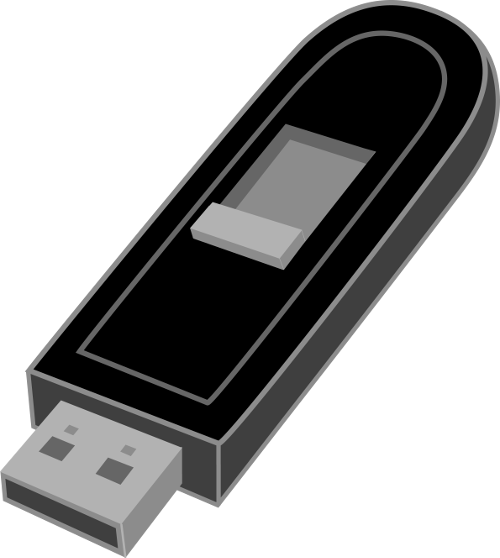
\includegraphics[width=3em]{img/usb}};
		\node[below right of=usb, node distance=1em] (db2) {
\includegraphics[width=1em]{img/db}};
		\draw[arrows=-latex,ultra thick] (db) -- node [above] {\small{copy}} (usb);
	
		\node[right of=usb, node distance=3.5cm](usb2) {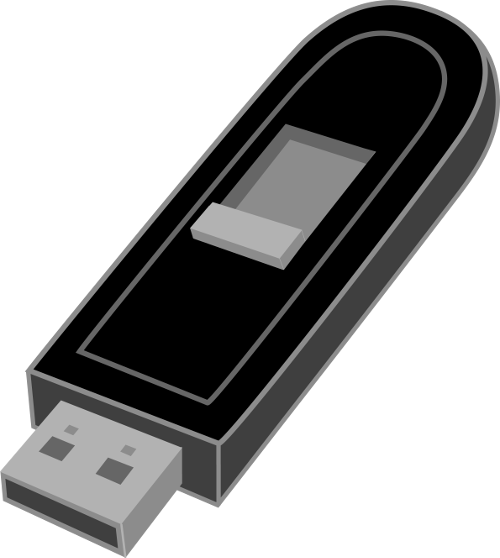
\includegraphics[width=3em]{img/usb}};
		\node[below right of=usb2, node distance=1em] (db4) {
\includegraphics[width=1em]{img/db}};
		\draw[arrows=-latex,ultra thick] (usb) -- node[above] (box) {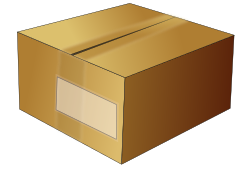
\includegraphics[width=4em]{img/box}} (usb2);
		\draw[arrows=-latex,ultra thick] (usb2) -- (pc2);
	}
	
	\visible<4->{
		\node at (10,0) {
\includegraphics[width=5cm]{img/no-fucks-given.jpg}};
	}
	\end{tikzpicture}
\end{figure}
\end{frame}

\section{Approach}

\begin{frame}{FMSync: Topology}
\begin{figure}
	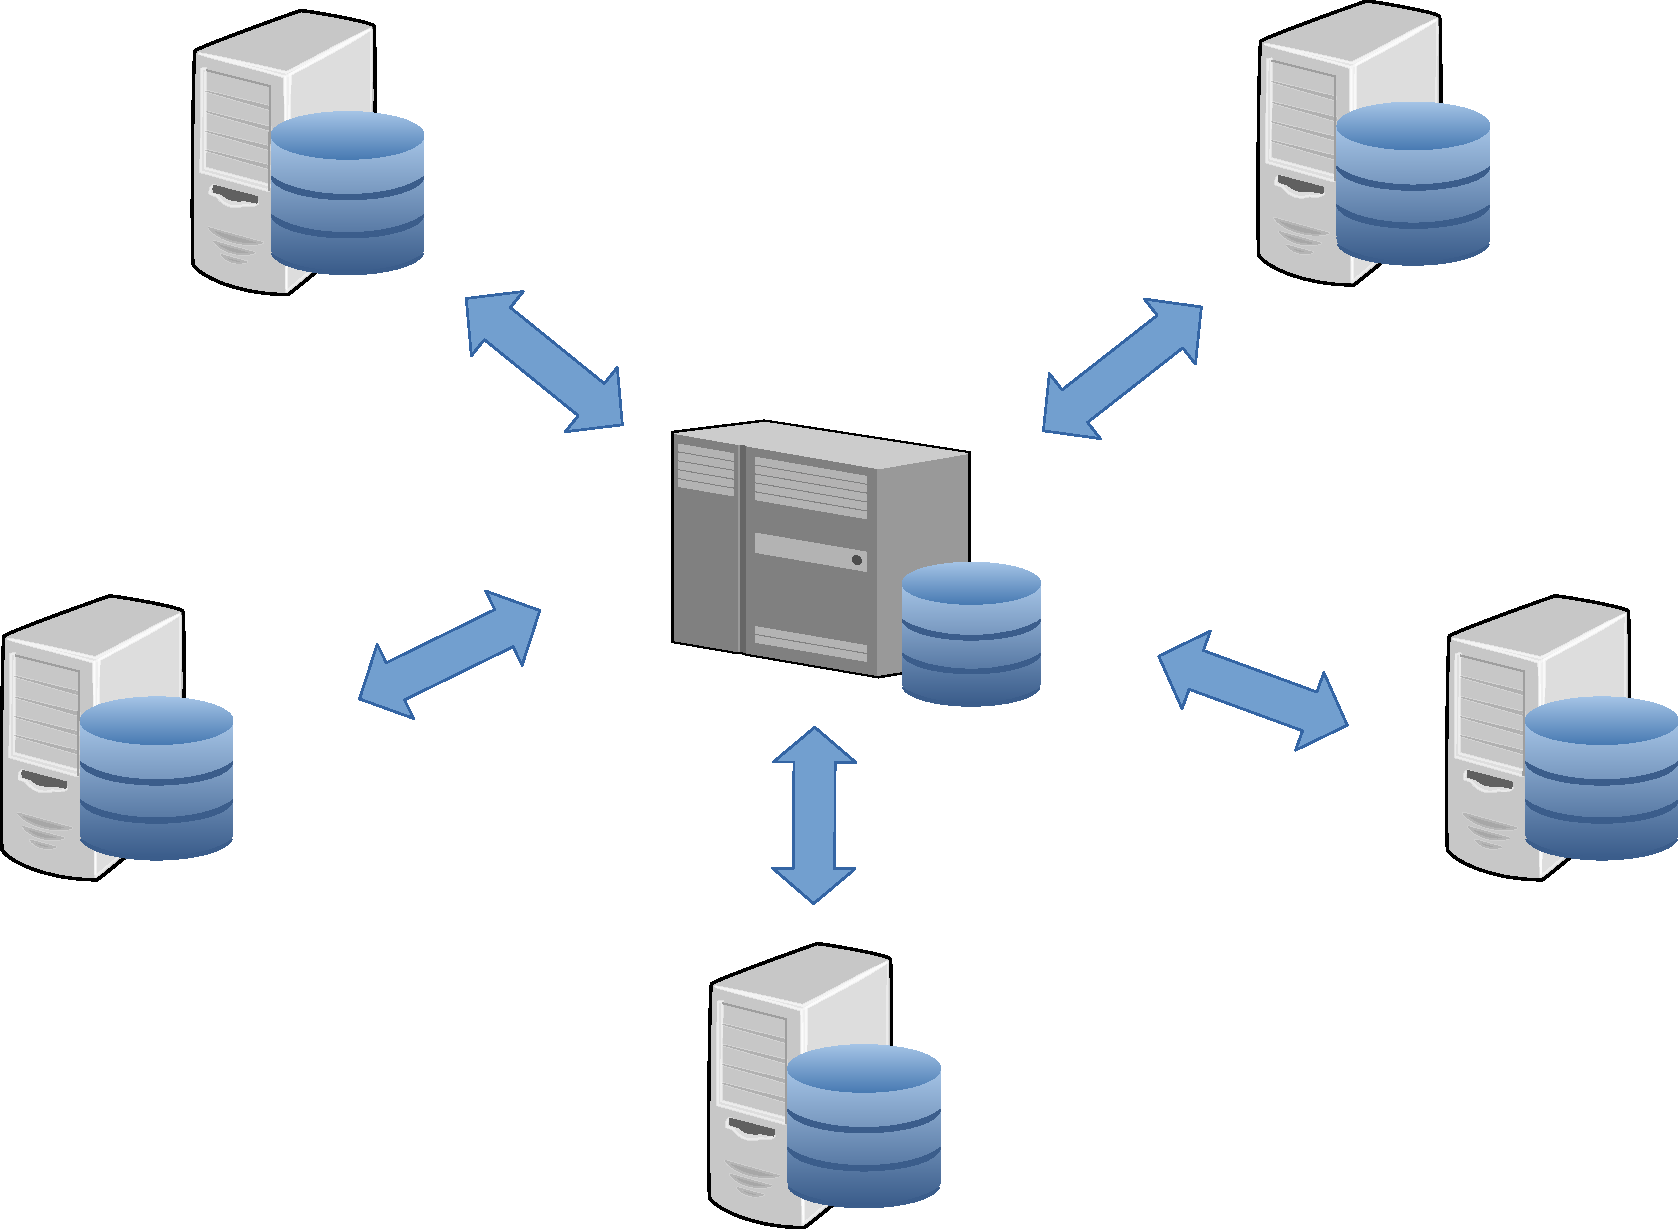
\includegraphics[height=.8\textheight]{img/topo.pdf}
\end{figure}
\end{frame}

\begin{frame}{Wait a second!}\large
Yo, Felix! 'Tis nuthin nu.\pause\bigskip

https://www.fmpromigrator.com/order/index.html
\normalsize

\begin{quote}
	\textbf{SymmetricDS} supports [\dots] \alert{Oracle}, \alert{MySQL}, MariaDB, \alert{PostgreSQL}, MS SQL Server (including Azure), IBM DB2 (UDB, iSeries, and zSeries), H2, HSQLDB, Derby, Firebird, Interbase, Informix, Greenplum, \alert{SQLite}, Sybase ASE, Sybase ASA (SQL Anywhere), Amazon Redshift, \alert{MongoDB}, and VoltDB databases.
\end{quote}\vspace{-1em}
\begin{flushright}
	\texttt{https://www.symmetricds.org/}
\end{flushright}
\end{frame}

\begin{frame}{FileMaker Solution}
\begin{figure}
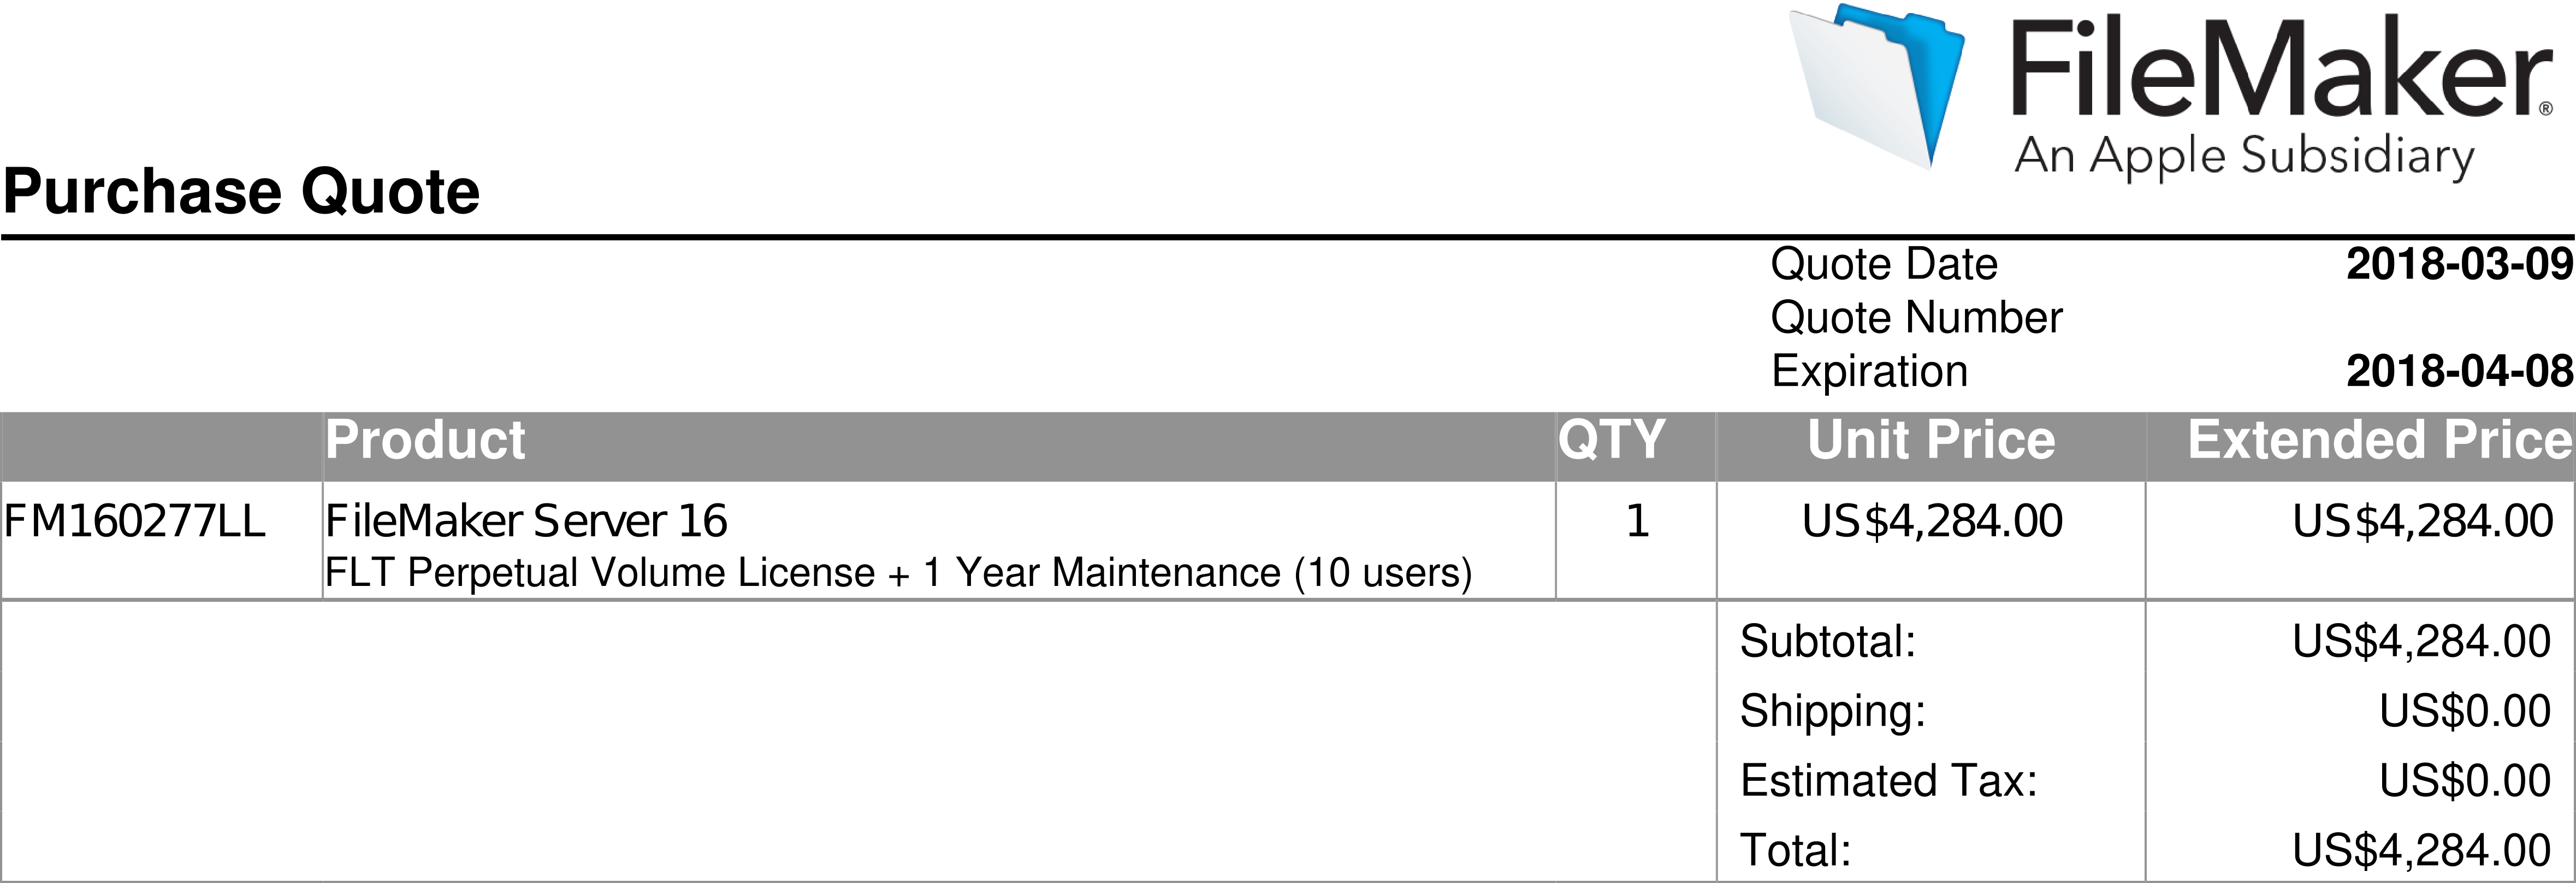
\includegraphics[width=\linewidth]{img/order.png}
\end{figure}\vspace{-2em}
\begin{itemize}
\item Proprietary, badly written software
\item Still totally not worth the price
\end{itemize}
\end{frame}

\begin{frame}{Our Solution}
open source (license!), free, platform independent (java)
\end{frame}

\begin{frame}{Why underestimation is bad}
\begin{center}
\begin{figure}
	
\includegraphics[width=\textwidth]{img/xkcd.png}
	\caption{I can relate to this. [xkcd.com/1831]}
\end{figure}
\end{center}
\end{frame}

\section{Implementation}

\begin{frame}{screenshot}
Inhalt...
\end{frame}

\begin{frame}{arachne}
bisschen zur zentralisierung
\end{frame}

\begin{frame}{Foreign Key Difficulty}\ttfamily\footnotesize
\begin{figure}
	\begin{tikzpicture}[/tikz/ampersand replacement=\&, label distance=.5cm,  every node/.style = {anchor= north west},every label/.style={font=\normalsize\sffamily\bfseries},
		table/.style={matrix of nodes, nodes in empty cells, column sep=-\pgflinewidth, row sep=-\pgflinewidth, nodes={draw,text depth=.5ex,text height=2ex,minimum width=2.5em}, row 1/.style={font=\bfseries, nodes={fill=lightgray!50,minimum height=1.7em}}}]
		
		\matrix(tl) [table, label=left:Type] {
			ID \& \dots \& FK\_Fabric \& \dots\only<1,3->{\\
			14 \& \dots \& \phantom{FKhl}3\phantom{abri} \& \dots}\only<2>{\\
			14 \& \dots \&|[fill=Green!40]| \phantom{FKhl}3\phantom{abri} \& \dots} \\};
		
		\matrix(fl) [table, label=left:Fabric, below=2.5cm of tl.south west,right] {
			ID \& color\&\dots\only<1,3->{\\
			3 \& brown\&\dots}
			\only<2>{\\
			|[fill=Green!40]| 3 \& brown\&\dots}\\};
	
	\visible<2>{\draw[ultra thick,->,color=OliveGreen!50!Green] (tl-2-3.south)-- (fl-2-1.north);}	
	
	\visible<3->{
		\draw[thick, dashed,gray] (5.75,-5.5) -- (5.75,0.5);
		\matrix(tr) [table, right=7cm of tl.north west, anchor=north west] {
			ID \& \dots \& FK\_Fabric \& \dots \\
			105 \& \dots \& \phantom{FKhl}x\phantom{abri} \& \dots\only<5,6>{\\
			106 \& \dots \& \phantom{FKhl}3\phantom{abri} \& \dots}\only<4>{\\
			|[fill=Green!40]| 106 \& \dots \& \phantom{FKhl}3\phantom{abri} \& \dots}\only<7->{\\
			106 \& \dots \&|[fill=red!40]|  \phantom{FKhl}3\phantom{abri} \& \dots} \\};
		
		\matrix(fr) [table, right=7cm of fl.north west, anchor=north west] {
			ID \& color\&\dots \\
			81 \& red\phantom{xt}\&\dots\only<6>{\\
			82 \& brown\&\dots}\only<5>{\\
			|[fill=Green!40]| 82 \& brown\&\dots}\only<7->{\\
			|[fill=red!40]| 82 \& brown\&\dots} \\};
	}
	\only<4>{\draw[ultra thick,->,color=OliveGreen!50!Green] (tl-2-4.east)-- node[above]{import} (tr-3-1.west);}
	\only<5>{\draw[ultra thick,->,color=OliveGreen!50!Green] (fl-2-3.east)-- node[above]{import} (fr-3-1.west);}
	\only<8>{\draw[ultra thick,->,color=red] (tr-3-3.north)--(7.75,0)node[above left]{\dots} ;}
	\end{tikzpicture}
\end{figure}
\end{frame}

\begin{frame}{Foreign Key Difficulty: Solution}\ttfamily\scriptsize
\begin{figure}
	\begin{tikzpicture}[/tikz/ampersand replacement=\&, every node/.style = {anchor= north west},every label/.style={font=\normalsize\sffamily\bfseries},
	table/.style={matrix of nodes, nodes in empty cells, column sep=-\pgflinewidth, row sep=-\pgflinewidth, nodes={draw,text depth=.5ex,text height=2ex,minimum width=2.5em}, row 1/.style={font=\bfseries, nodes={fill=lightgray!50,minimum height=1.7em}}}]
	
	\matrix(typea) [table, label=left:\rotatebox{90}{Type}] {
		ID \& \dots \& FKF \& FKP\only<1>{\\
		5 \& \dots \& 29 \& 8}\only<2->{\\
		5 \& \dots \&|[fill=violet!40]| 29 \&|[fill=orange!40]| 8} \\};
		
	\matrix(fabrica) [table, label=left:\rotatebox{90}{Fabric}, below left=1cm of typea.south] {
		ID \& \dots \& FKC \only<1>{\\
		29 \& \dots \& 3 }\only<2->{\\|[fill=violet!40]|
		29 \& \dots \&|[fill=NavyBlue!40]| 3}\\};
		
	\matrix(placea) [table, label=left:\rotatebox{90}{Place}, right=5em of fabrica.north east,anchor=north west] {
		ID \& \dots \only<1>{\\
		8 \& \dots}\only<2->{\\|[fill=orange!40]|
		8 \& \dots}\\};
	
	\matrix(colora) [table, label=left:\rotatebox{90}{Color}, below right=1cm of fabrica.south west] {
		ID \& color\&\dots\only<1>{\\
		3 \& brown\&\dots}\only<2->{\\|[fill=NavyBlue!40]| 
		3 \& brown\&\dots}\\};
	
	\visible<3->{
		\draw[thick, dashed, gray] (5,-5.5) -- (5,0.5);
		\visible<4->{
			\matrix(colorb) [table, label=left:\rotatebox{90}{Color}, right=5cm of colora] {
				ID \& color\&\dots\only<8-12>{\\
				19 \& brown\&\dots}\only<4>{\\|[fill=Green!40]| 
				19 \& brown\&\dots}\only<5-7,13>{\\|[fill=NavyBlue!40]| 
				19 \& brown\&\dots}\\};
		}
		\visible<6->{
			\matrix(fabricb) [table, label=left:\rotatebox{90}{Fabric}, above left=1cm of colorb, anchor=south west] {
				ID \& \dots \& FKC\only<6>{\\|[fill=Green!40]|
				45 \& \dots \& 19}\only<8-12>{\\|[fill=violet!40]|
				45 \& \dots \& 19}\only<7,13>{\\|[fill=violet!40]|
				45 \& \dots \&|[fill=NavyBlue!40]| 19}\\};
		}
		\visible<9->{
			\matrix(placeb) [table, label=left:\rotatebox{90}{Place}, right=5em of fabricb.north east,anchor=north west] {
				ID \& \dots\only<9>{\\|[fill=Green!40]|
				67 \& \dots}\only<10-13>{\\|[fill=orange!40]|
				67 \& \dots}\\};
		}
		\visible<11->{
			\matrix(typeb) [table, label=left:\rotatebox{90}{Type}, above right=1cm of fabricb, anchor=south] {
				ID \& \dots \& FKF \& FKP\only<11>{\\|[fill=Green!40]|
				98 \& \dots \& 45 \& 67}\only<12->{\\
				98 \& \dots \&|[fill=violet!40]| 45 \&|[fill=orange!40]| 67} \\};
		}
	}
	
	\only<2->{
		\draw[ultra thick,->,color=violet] (typea-2-3.south)-- (fabrica-2-1.north);
		\draw[ultra thick,->,color=orange] (typea-2-4.south)-- (placea-2-1.north);
		\draw[ultra thick,->,color=NavyBlue] (fabrica-2-3.south)-- (colora-2-1.north);
	}
	\only<4>{\draw[ultra thick,->,color=OliveGreen!50!Green] (colora-2-3.east)-- node[above]{import} (colorb-2-1.west);}
	\only<6>{\draw[ultra thick,->,color=OliveGreen!50!Green,bend right=25] (fabrica-2-3.south east) to node[above]{import} node[below,color=NavyBlue]{\textbf{FKC=19}} (fabricb-2-1.south west);}
	\only<7,13>{\draw[ultra thick,->,color=NavyBlue](fabricb-2-3.south) -- (colorb-2-1.north);}
	\only<9>{\draw[ultra thick,->,color=OliveGreen!50!Green,bend right=20] (placea-2-2.south east) to node[above]{import} (placeb-2-1.south west);}
	\only<11>{\draw[ultra thick,->,color=OliveGreen!50!Green] (typea-2-4.east) to node[above]{import} node[below]{\textbf{\textcolor{violet}{FKF=45}}\quad\textbf{\textcolor{orange}{FKP=67}}}  (typeb-2-1.west);}
	\only<12->{\draw[ultra thick,->,color=violet](typeb-2-3.south) -- (fabricb-2-1.north);}
	\only<12->{\draw[ultra thick,->,color=orange](typeb-2-4.south) -- (placeb-2-1.north);}
	\end{tikzpicture}
\end{figure}
\end{frame}

\begin{frame}[plain,standout]
\vfill
\begin{center}\Large
Thank you very much for your attention!\\\bigskip
https://github.com/horle/fmsync
Questions?
\end{center}\vfill
\end{frame}

\maketitle

\end{document}
